\documentclass[preprint]{aastex}

\usepackage{float}
\bibliographystyle{apj}

\begin{document}

\title{The dimensionality of stellar abundance space using red clump stars from APOGEE}
\author{Natalie Price-Jones, supervised by Professor Jo Bovy}

\begin{abstract}
Recent spectroscopic surveys have provided abundant data on stars in the Milky Way. I will analyze a subset of data from the Apache Point Observatory Galactic Evolution Experiment (APOGEE) survey, in the form of red clump stars. These metal-enriched stars offer a complex abundance space to explore, which I will do by studying the spectra themselves, rather than derived abundances. This direct use of the spectra facilitates the characterization of errors and systematic effects in interpretation of absorption features. An understanding of these uncertainties allows accurate investigation of the multi-dimensional abundance space, which may reveal trends in abundances with stellar age and position throughout the Milky Way. Tracing out a star's abundances and these possible trends offers a way to investigate the dynamical and formation history of the Milky Way.

%These trends may also provide a comparative method to assess uncertainties associated with current abundance calculations.

\end{abstract}

\section{Introduction}
\label{sec:back}
A star's history, from its formation environment to its migratory motions, can be traced through its composition. Measuring elemental abundances from stellar spectra establishes this composition. However, current methods for calculating these abundances require robust theoretical models and complete understanding of measurement uncertainties. At present, these methods still exhibit systematic trends with other stellar properties, such as effective temperature $T_{\rm eff}$ or surface gravity $\log(g)$ \citep{holtzman2015}. Removing these contaminating effects from abundance calculations entirely may reveal statistically significant correlations between abundances and stellar age or location within a galaxy. 

Recent large-volume spectroscopic survey data from the Apache Point Observatory Galactic Evolution Experiment (APOGEE, \citealt{APOGEE}), upcoming data from the Gaia mission \citep{GAIA} and other large spectroscopic surveys will offer rich spectral information about hundreds of thousands of stars. This data is a prime opportunity for abundance analysis. To take advantage of this, I will develop an efficient method for investigating abundance space \citep{openclusters}. The method, described in \S\ref{sec:methods}, uses spectra directly, rather than quantities derived by fitting multi-parameter model spectra. This reduces complexity in calculations of uncertainty, and is less sensitive to the systematic effects of other stellar properties than traditional methods. This will allow for a more accurate investigation the dimensionality of abundance space for a sample of stars, including probing the relative significance of particular elements. I will apply this method to spectra from APOGEE and investigate the dimensionality of the sample in abundance space. An understanding of trends in this space may place constraints on what chemical processes contributed to the formation of populations of stars. This in turn may reveal elements of the Milky Way's star formation history or trace how stars moved through the Milky Way after their formation.

%Binning stars with similar abundance values in all elements into mono-abundance populations (MAPs), allows us to find locational trends when stars in the same MAP are located on-sky. 
 



%This project will investigate the multidimensional elemental abundance space of red clump stars from the APOGEE survey. We will investigate the significance of each of the 15 elements indentified by APOGEE as having measurable abundances. Previous work \citep{bovy2015} has found that correlating calculated alpha-element abundances [$\alpha$/Fe] to iron abundances [Fe/H] reveals two distinct populations: a main trendline, with another population that has an enhancement above this line in $\alpha$ elements (O, Mg, Si, S, Ca, Ti): see Figure \ref{fig:abun}. We will investigate the $\alpha$ elements individually, as well as the other 8 elemental abudances identified by APOGEE, for similar correlations, and trace where these stars are located within the galaxy (radially and vertically). Stars falling into the same small bins in all elemental abundances we call mono abundance populations (MAPS). Locating such populations may make it possible to trace motion of stars over the course of their lifetimes, knowing that stars with similar elemental abudances likely had similar formation environments.

\section{Data Set}
\label{sec:data}
This work will analyze the spectra of a sample of red clump stars from APOGEE's Data Release 12. These stars are selected as belonging to the red clump according to cuts in gravity, effective temperature, and metallicity, and leave us with an initial sample of 19936 stars \citep{bovy2014}. These stars trace, to some extent, the stellar population of the Milky Way through the volume of the APOGEE survey, which covers a significant fraction of the Milky Way’s disk. Data on these stars comes in the form of infrared (H-band) spectra covering a wavelength range from 1.514 $\mu$m to 1.696 $\mu$m (with some small nm gaps between detectors, \citealt{APOGEE}). APOGEE's DR12 pipeline provides data on abundances of 15 elements (C, N, O, Na, Mg, Al, Si, S, K, Ca, Ti, V, Mn, Fe, Ni) as well as effective temperature ($T_{\rm eff}$), surface gravity ($\log(g)$), overall metallicity ($Z$), and alpha-element enhancements ([$\alpha$/Fe])\citep{holtzman2015}. I will analyze all 15 of these elements.

\section{Methods}
\label{sec:methods}
Starting with our sample of APOGEE spectra, I will perform empirical fits to remove non-abundance stellar properties. Flux values from each spectrum at a given pixel $p$ $(F(p))$ are fit with a low order polynomial in $T_{\rm eff}$, $\log(g)$ and $Z$, so some function for flux is found: $f(p,T_{\rm eff},\log(g),Z)$ (see Figure \ref{fig:fit} for an example fit). At pixels ($p_\mathrm{X}$) known to host absorption features for an element X, residuals are calculated from the fit: $\delta = F(p_\mathrm{X}) - f(p_\mathrm{X},T_{\rm eff},\log(g),Z)$. Residuals for element X pixels are weighted by normalized window functions which trace each X absorption feature and are then summed for each spectrum. This identifies scatter in element X for each star, since other systematic effects have been removed by the fit. It remains to characterize what portion of this scatter is due to measurement noise or intrinsic effects particular to the element. The measurement noise can be determined from uncertainties in $F(p)$, and both measurement noise and intrinsic element scatter can be estimated from a sample of open cluster stars \citep{meszaros2015}, which should all have similar abundance properties. The remaining scatter for each star after these effects have been accounted for will represent some variation in the 15 dimensional abundance space (see Figure \ref{fig:resid} for a histogram showing the spread in element residuals compared with measurement uncertainty). The importance of these variations will be investigated through principal component analysis (PCA), finding the linear combinations of element residuals with the most significant variance.

\section{Timeline}
\label{sec:timeline}

\begin{itemize}
\item Nov 2015, Q: Can I see scatter in residuals of individual elements above our level of intrinsic and measurement uncertainty?
\begin{itemize}
\item Characterize measurement scatter by drawing from a Gaussian determined by the uncertainty in flux measurements.
\item Fit open clusters (from \citealt{meszaros2015}) in $T_{\rm eff}$ according to the outline in \S3 and take residuals from this fit as representative of intrinsic abundance scatter.
\end{itemize}
\item Dec 2015, Q: What is the dimensionality of abundance space for all elements? Which elements are most significant for distinguishing stars?
\begin{itemize}
\item Use principal component analysis to identify elements of primary importance and the number of dimensions that are not due to noise.
\end{itemize}
\item Jan/Feb 2016, Q: Is there any positional dependence of populations in small bins in the remaining dimensions of abundance space?
\begin{itemize}
\item Collect stars from small bins in the multidimensional residual space and plot their radial and vertical positions.
\item Determine if stars belonging to different bins inhabit different sections of the galaxy, as well as positional variations for stars within a bin.
\end{itemize}
\item Mar/Apr 2016, Q: Can I understand the reasons certain elements may be more significant after PCA by modeling spectra?
\begin{itemize}
\item Create model spectra by varying abundances of the 15 elements.
\item Perform fitting described in \S\ref{sec:methods} and compare with fitting done on APOGEE data. Ascertain whether model spectra created with derived abundances for the red clump stars can reproduce residual results from the data set.
\end{itemize}
\end{itemize}

\bibliography{cite}

\begin{figure}[H]
\centering
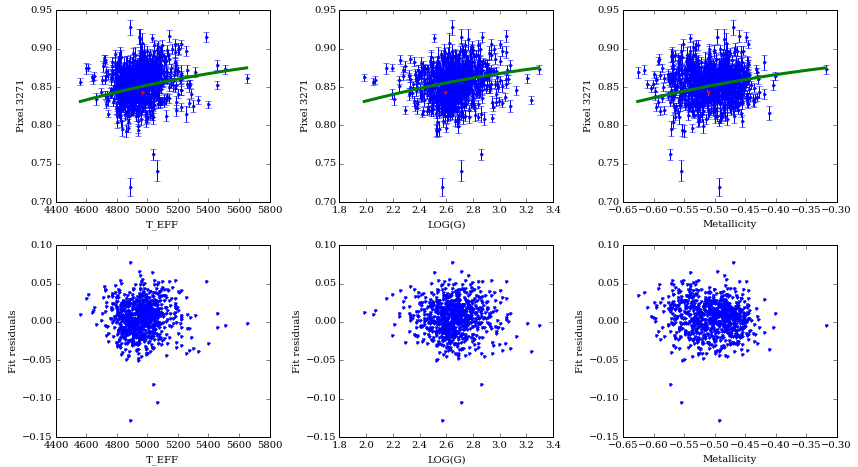
\includegraphics[width = \linewidth]{pix3271fit.png}
\caption{Sample second order fit to flux values at pixel 3271 for each star in the sample. Blue dots are the flux values, the green line is the simultaneous fit second order fit in three parameters: $T_{\rm eff}$, $\log(g)$ and $Z$. Red dots indicate points with large uncertainty (>0.1 in the normalized flux units). These points were plotted without error bars but are still included in the fit. Each upper panel is the fit plotted against one of its dimensions, the lower panels are the residuals from these results, assumed to be due to variations in abundances. This pixel corresponds to an absorption feature for Mg.}
\label{fig:fit}
\end{figure}

\begin{figure}[H]
\centering
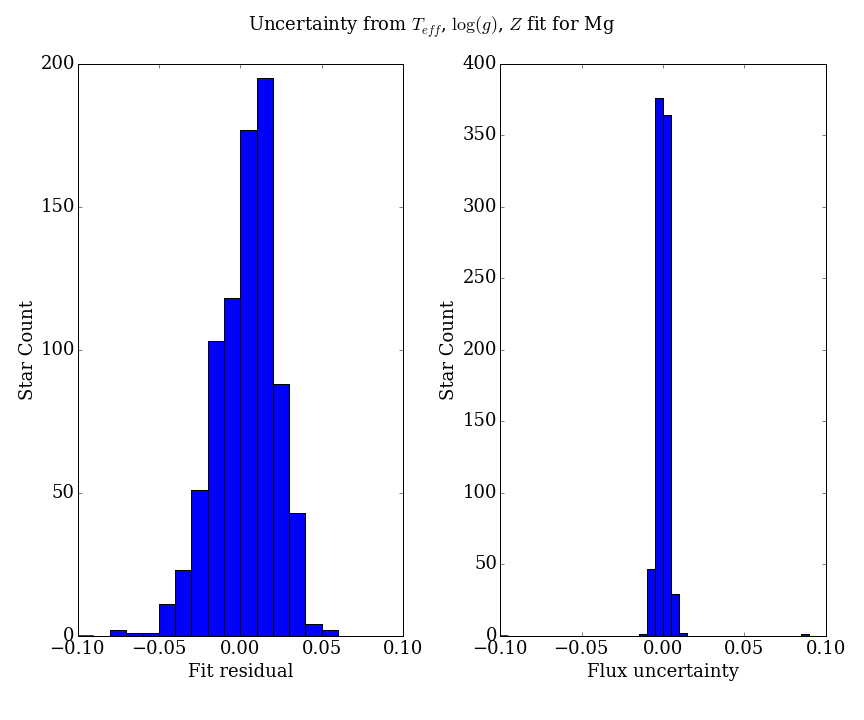
\includegraphics[width = \linewidth]{Mg_residuals.png}
\caption{The left panel shows a histogram of the weighted residuals for several pixels associated with Mg absorption from each stellar spectrum. The right panel is a histogram of the fractional uncertainty in the flux value. This is calculated by drawing randomly from a normal distribution with a standard deviation of the measurement uncertainty at each relevant pixel and dividing it by the flux value at that pixel. These fractional results are then weighted and summed in the same way as the residual values to produce the histogram in the right panel.}
\label{fig:resid}
\end{figure}

\end{document}